\chapter{Thermodynamics and Finite Size Scaling}


\begin{figure}[h]
	\centering
	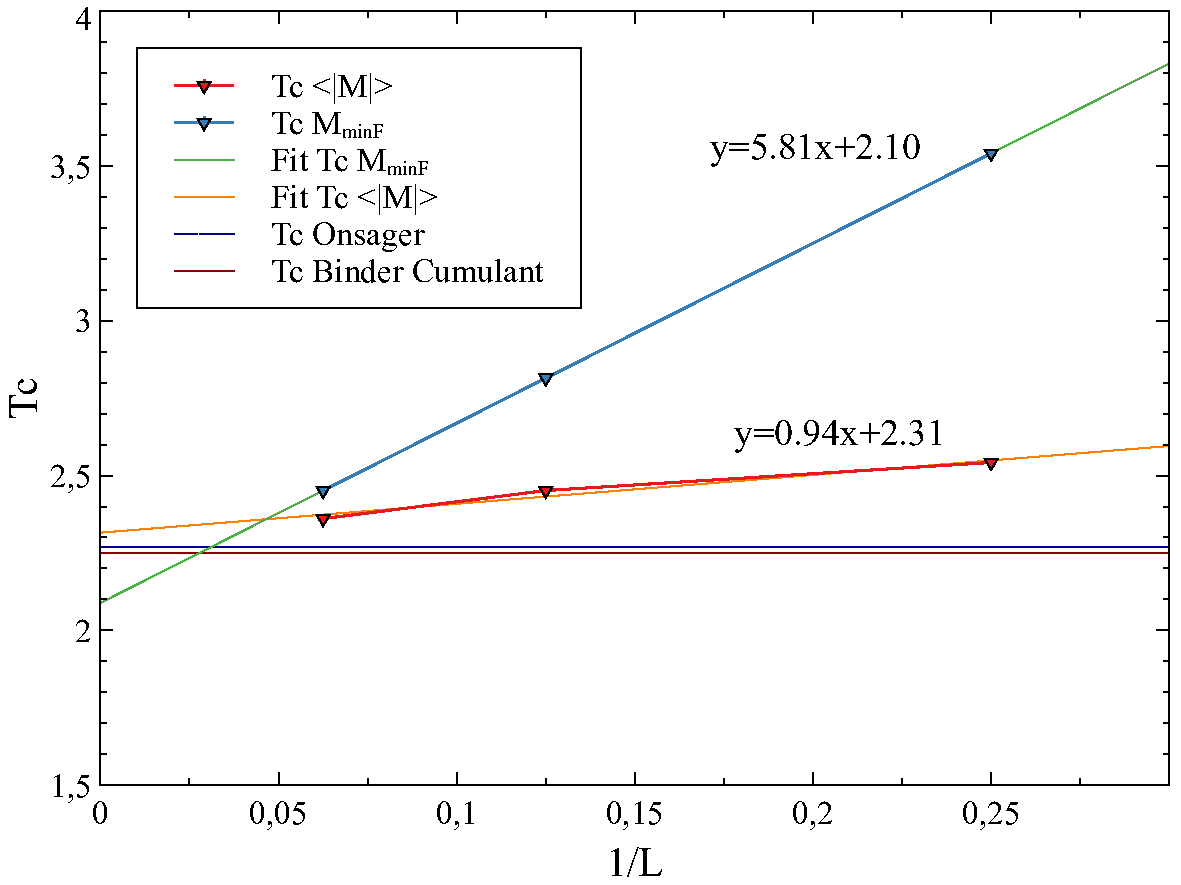
\includegraphics[scale=0.45]{thermodynamics/thermodynamics_finite_size_01.pdf}
	\caption{Scheme of how the Flat Scan Sampling works.}
\end{figure}

\begin{figure}[h]
	\centering
	\subfigure[]{
		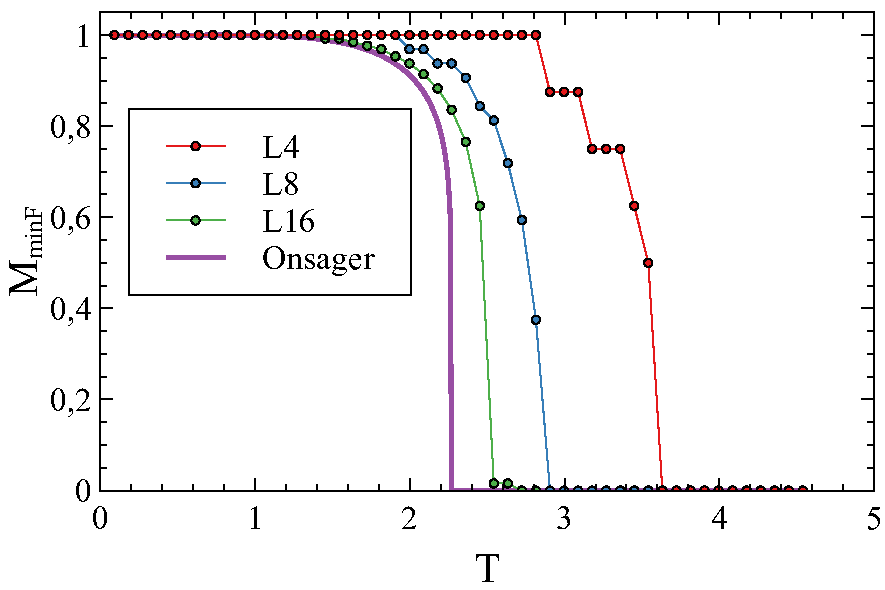
\includegraphics[scale=0.49]{thermodynamics/thermodynamics_finite_size_02.pdf}
	}	
	\subfigure[]{
		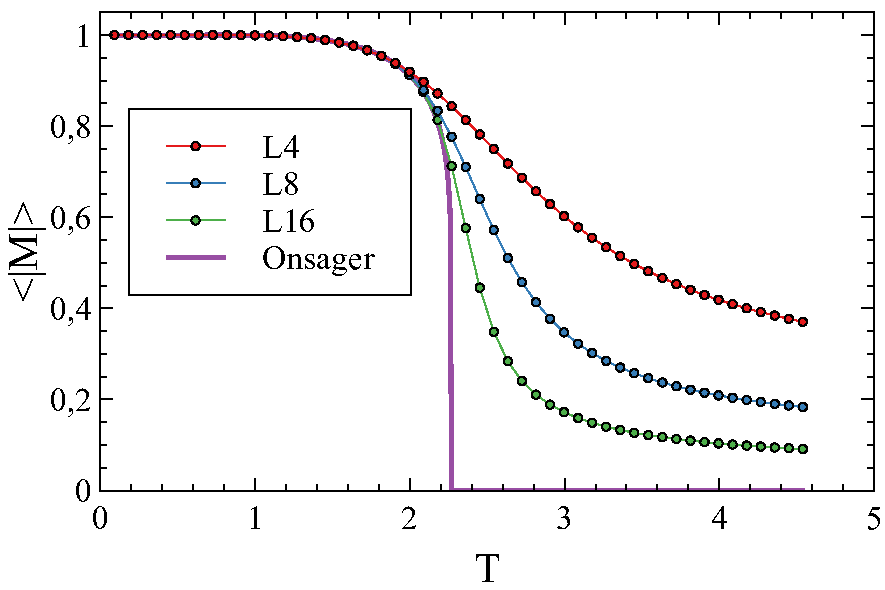
\includegraphics[scale=0.49]{thermodynamics/thermodynamics_finite_size_03.pdf}
	}	
	
	\subfigure[]{
		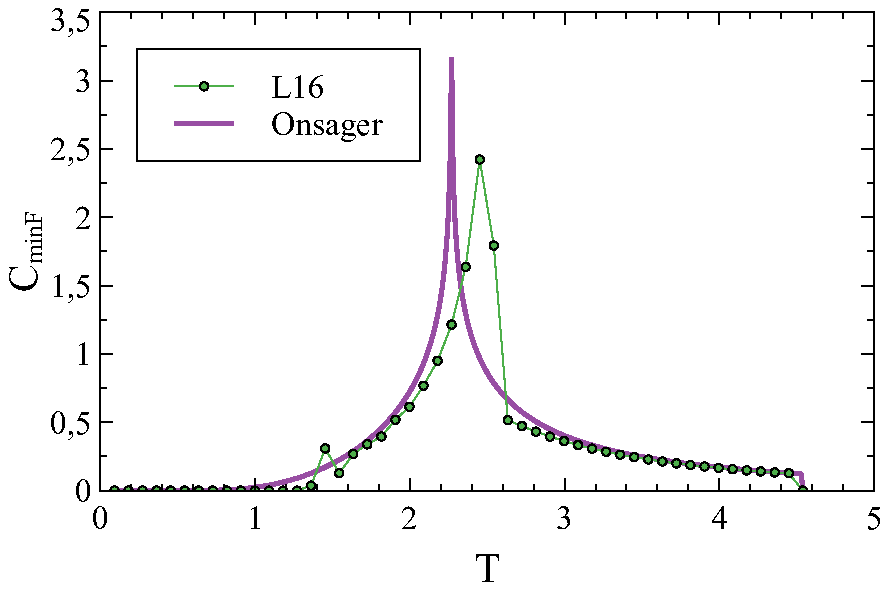
\includegraphics[scale=0.49]{thermodynamics/thermodynamics_finite_size_04.pdf}
	}	
	\subfigure[]{
		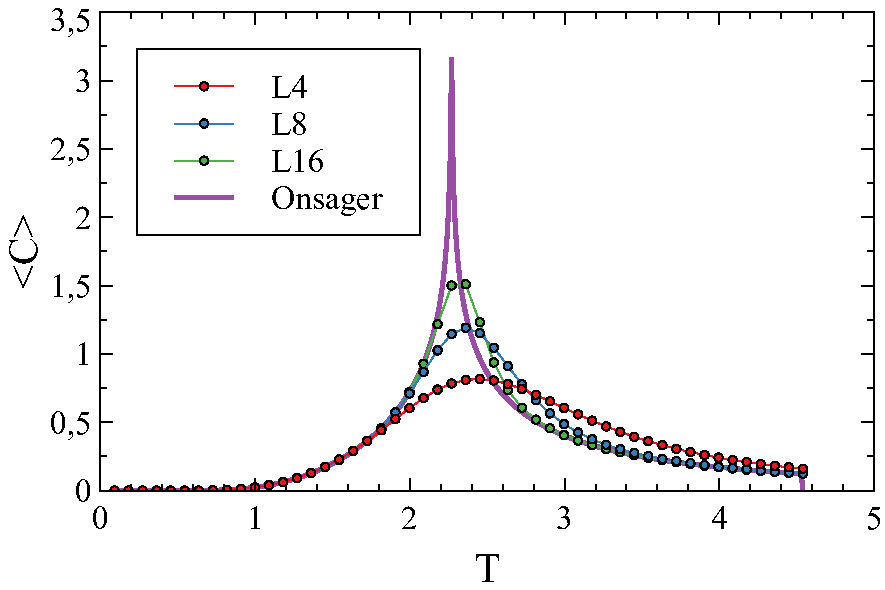
\includegraphics[scale=0.49]{thermodynamics/thermodynamics_finite_size_05.pdf}
	}	
	
	\caption{Scheme of how the Flat Scan Sampling works.}
\end{figure}


\begin{figure}[h]
	\centering
	\subfigure[]{
			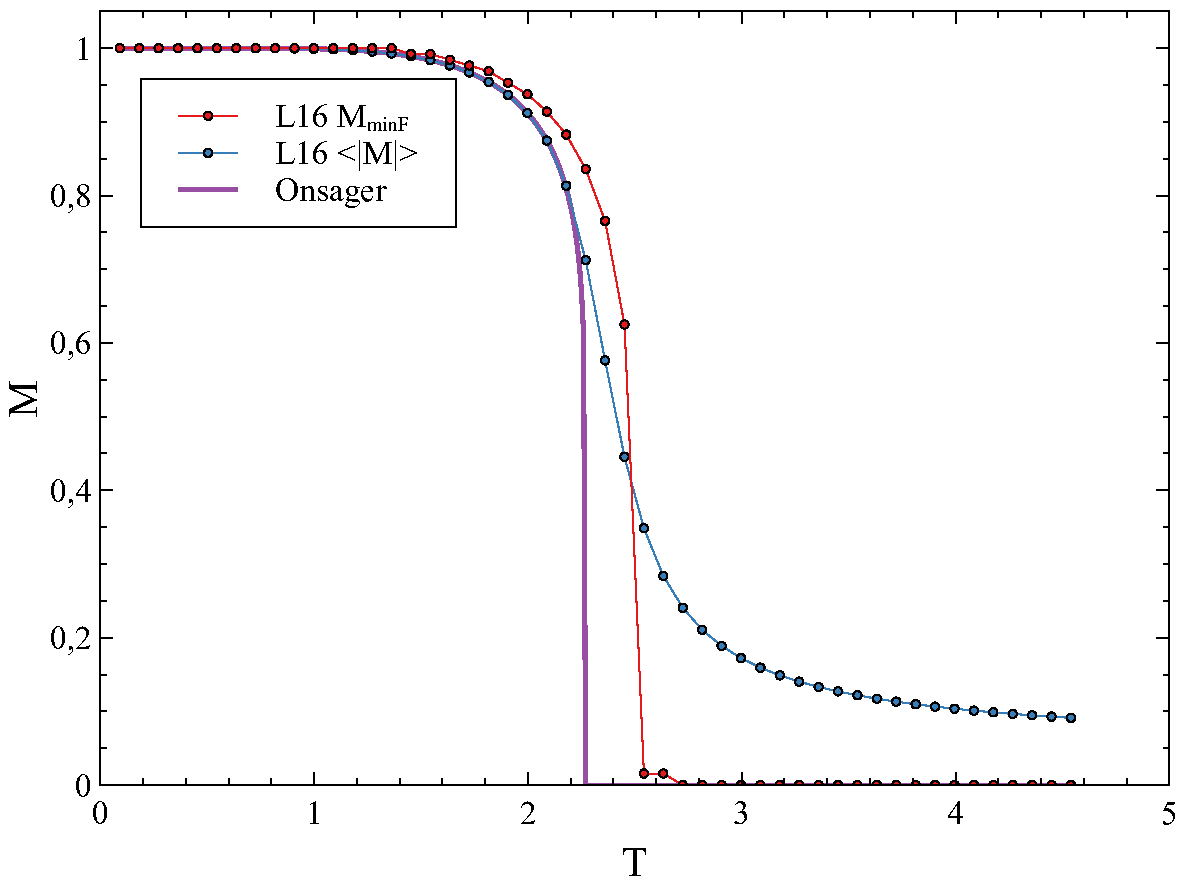
\includegraphics[scale=0.37]{thermodynamics/thermodynamics_finite_size_06.pdf}
	}
	\subfigure[]{
		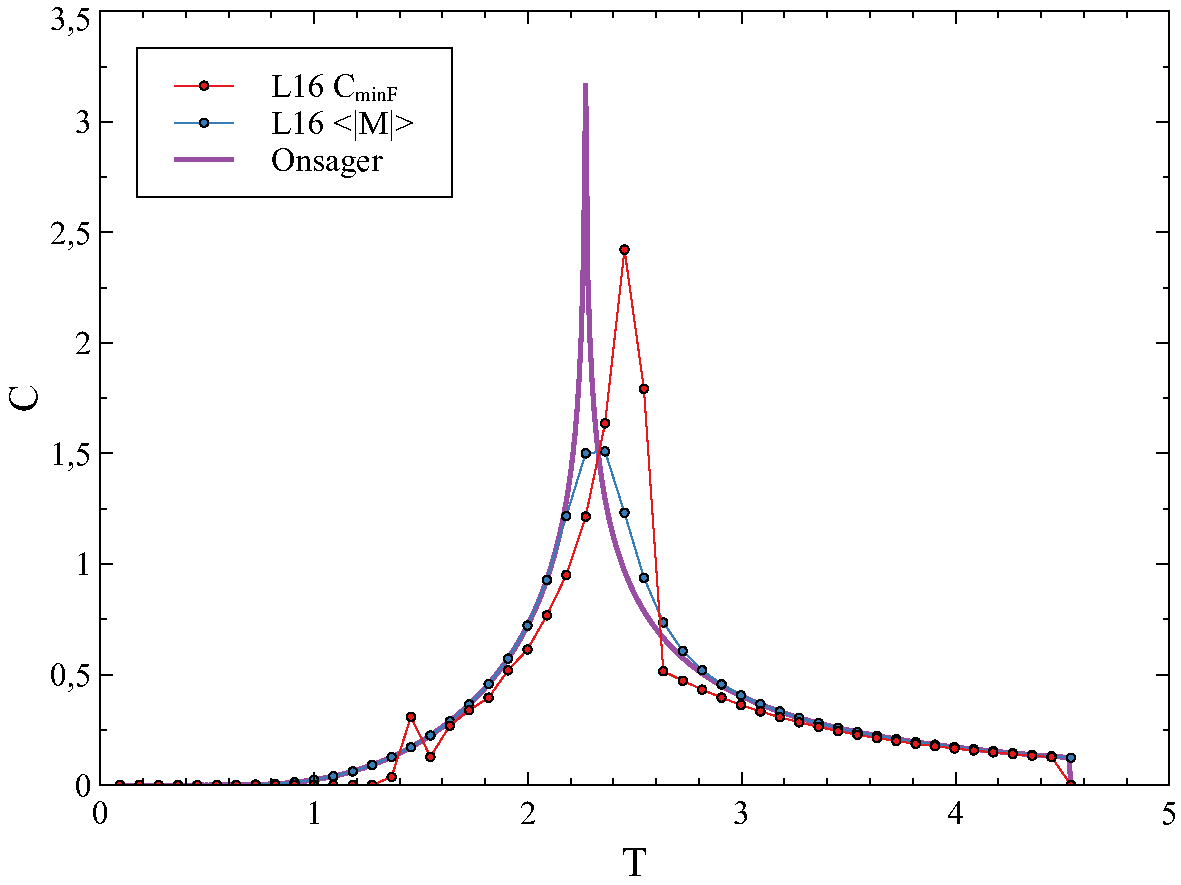
\includegraphics[scale=0.37]{thermodynamics/thermodynamics_finite_size_07.pdf}
	}
	
	\caption{Scheme of how the Flat Scan Sampling works.}
\end{figure}


